This test case is identical to Case~1c described above, except for the use of the Beta distribution for the vulnerability functions instead of the lognormal distribution. The conditional loss ratio exceedance matrix in this case is populated by evaluating the complementary cumulative distribution function (CCDF) of the Beta distribution at each of the prescribed intensity levels, for the set of loss ratios.

\begin{table}[htbp]

\centering
\begin{tabular}{ l c c c c c c c c c }

\hline
\rowcolor{anti-flashwhite}
\bf{LR | PGA} & \bf{0.05g} & \bf{0.20g} & \bf{0.40g} & \bf{0.60g} & \bf{0.80g} & \bf{1.00g} & \bf{1.20g} & \bf{\dots} & \bf{2.00g} \\
\hline
\bf{0.01} & 0.496 & 1.000 & 1.000 & 1.000 & 1.000 & 1.000 & 1.000 & \dots & 1.000 \\
\bf{0.04} & 0.000 & 0.485 & 0.999 & 1.000 & 1.000 & 0.999 & 0.996 & \dots & 1.000 \\
\bf{0.10} & 0.000 & 0.000 & 0.472 & 0.959 & 0.984 & 0.987 & 0.982 & \dots & 1.000 \\
\bf{0.20} & 0.000 & 0.000 & 0.000 & 0.468 & 0.844 & 0.928 & 0.944 & \dots & 1.000 \\
\bf{0.33} & 0.000 & 0.000 & 0.000 & 0.032 & 0.473 & 0.778 & 0.871 & \dots & 1.000 \\
\bf{0.50} & 0.000 & 0.000 & 0.000 & 0.000 & 0.100 & 0.500 & 0.738 & \dots & 1.000 \\
\bf{0.67} & 0.000 & 0.000 & 0.000 & 0.000 & 0.006 & 0.222 & 0.563 & \dots & 0.999 \\
\bf{0.80} & 0.000 & 0.000 & 0.000 & 0.000 & 0.000 & 0.072 & 0.394 & \dots & 0.995 \\
\bf{0.90} & 0.000 & 0.000 & 0.000 & 0.000 & 0.000 & 0.013 & 0.234 & \dots & 0.976 \\
\bf{0.96} & 0.000 & 0.000 & 0.000 & 0.000 & 0.000 & 0.001 & 0.115 & \dots & 0.925 \\
\bf{0.99} & 0.000 & 0.000 & 0.000 & 0.000 & 0.000 & 0.000 & 0.038 & \dots & 0.822 \\
\bf{1.00} & 0.000 & 0.000 & 0.000 & 0.000 & 0.000 & 0.000 & 0.000 & \dots & 0.000 \\
\hline
\end{tabular}

\caption{Conditional loss ratio exceedance matrix for classical risk test case 1d}
\label{tab:lrem-bt-tax1-nzcov}
\end{table}

The loss ratio exceedance matrix in this case is shown in Table~\ref{tab:lrem-bt-tax1-nzcov}.

The loss curve thus calculated above is compared with the loss curve obtained using the OpenQuake classical PSHA based risk calculator in Figure~\ref{fig:lc-cr-1d}.

\begin{figure}[htbp]
\centering
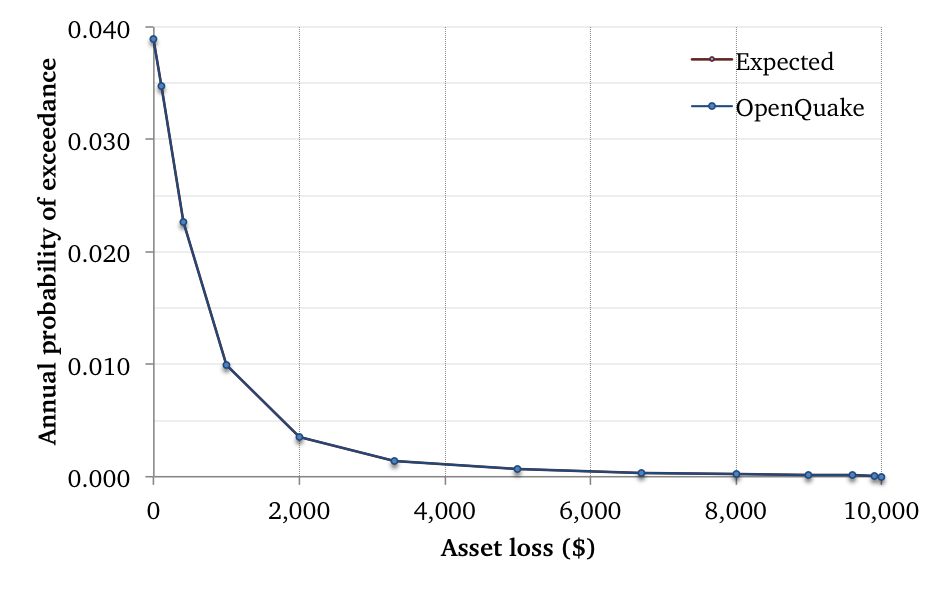
\includegraphics[width=12cm]{qareport/figures/fig-lc-cr-1d}
\caption{Loss curve comparison for classical risk test case 1d}
\label{fig:lc-cr-1d}
\end{figure}

The area under the annual loss exceedance curve gives the average annual loss.